\documentclass[border=4pt]{standalone}
\usepackage[sfdefault,lining]{FiraSans}
\usepackage[T1]{fontenc}
\usepackage{amsmath,amssymb}
\usepackage{tikz}
\usetikzlibrary{arrows.meta,positioning,calc}
\definecolor{gaC}{HTML}{2A78D6}\definecolor{tsC}{HTML}{EB6834}\definecolor{maC}{HTML}{1BAF7A}
\definecolor{ink}{HTML}{0B0B0B}\definecolor{ink2}{HTML}{52514E}\definecolor{muted}{HTML}{898781}
\definecolor{gridc}{HTML}{E1E0D9}\definecolor{addC}{HTML}{1BAF7A}\definecolor{remC}{HTML}{E34948}
\begin{document}
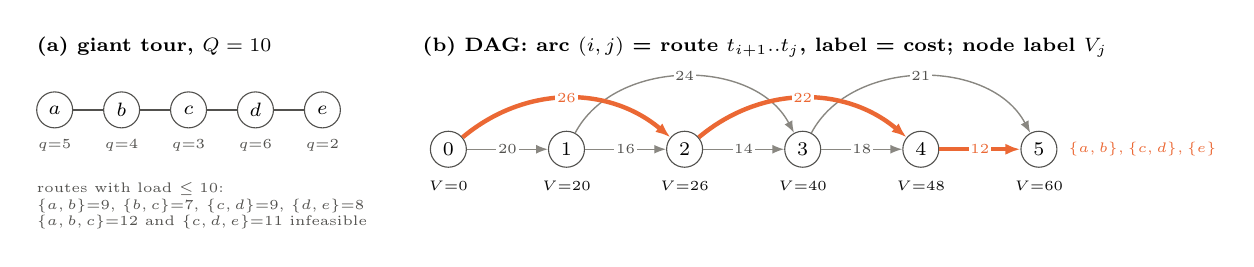
\begin{tikzpicture}[x=1cm,y=1cm,font=\scriptsize,
  nd/.style={circle,draw=ink2,fill=white,minimum size=13pt,inner sep=0pt},
  arc/.style={-{Latex[length=1.5mm]},draw=muted,line width=0.5pt},
  best/.style={-{Latex[length=1.9mm]},draw=tsC,line width=1.6pt},
  lab/.style={font=\tiny,fill=white,inner sep=0.6pt,text=ink2}]
\node[anchor=west,font=\scriptsize\bfseries] at (-0.35,2.05) {(a) giant tour, $Q=10$};
\foreach \x/\c/\q in {0/a/5,0.85/b/4,1.7/c/3,2.55/d/6,3.4/e/2} {
  \node[nd] (g\c) at (\x,1.25) {$\c$}; \node[font=\tiny,ink2] at (\x,0.8) {$q{=}\q$};}
\foreach \u/\w in {a/b,b/c,c/d,d/e} \draw[ink2,line width=0.5pt] (g\u)--(g\w);
\node[font=\tiny,ink2,align=left,anchor=north west] at (-0.35,0.45) {routes with load $\le 10$:\\ $\{a,b\}{=}9$, $\{b,c\}{=}7$, $\{c,d\}{=}9$, $\{d,e\}{=}8$\\ $\{a,b,c\}{=}12$ and $\{c,d,e\}{=}11$ infeasible};
\node[anchor=west,font=\scriptsize\bfseries] at (4.55,2.05) {(b) DAG: arc $(i,j)$ = route $t_{i+1}..t_j$, label = cost; node label $V_j$};
\foreach \i/\V in {0/0,1/20,2/26,3/40,4/48,5/60} {
  \node[nd] (h\i) at (5.0+1.5*\i,0.75) {\i}; \node[font=\tiny,ink] at (5.0+1.5*\i,0.28) {$V{=}\V$};}
\foreach \i/\j/\c in {0/1/20,1/2/16,2/3/14,3/4/18} \draw[arc] (h\i)--(h\j) node[lab,midway] {\c};
\foreach \i/\j/\c in {1/3/24,3/5/21} \draw[arc] (h\i) to[bend left=62] node[lab,pos=0.5] {\c} (h\j);
\draw[best] (h0) to[bend left=40] node[lab,midway,text=tsC] {26} (h2);
\draw[best] (h2) to[bend left=40] node[lab,midway,text=tsC] {22} (h4);
\draw[best] (h4)--(h5) node[lab,midway,text=tsC] {12};
\node[font=\tiny,tsC,anchor=west] at (12.75,0.75) {$\{a,b\},\{c,d\},\{e\}$};
\end{tikzpicture}
\end{document}
